\documentclass[
	12pt,
	oneside,
	a4paper,
	english,
	french,
	spanish,
	brazil,
	]{abntex2}

\usepackage{lmodern}
\usepackage[T1]{fontenc}
\usepackage[utf8]{inputenc}
\usepackage{indentfirst}
\usepackage{color}
\usepackage{graphicx}
\usepackage{microtype}

\usepackage[brazilian,hyperpageref]{backref}
\usepackage[alf]{abntex2cite}

\graphicspath{{./images/}}

\renewcommand{\backrefpagesname}{Citado na(s) página(s):~}
\renewcommand{\backref}{}
\renewcommand*{\backrefalt}[4]{
	\ifcase #1
		Nenhuma citação no texto.
	\or
		Citado na página #2.
	\else
		Citado #1 vezes nas páginas #2.
	\fi}

\titulo{Primeiro Trabalho Prático}
\autor{Tulio Brunoro de Souza}
\local{Vitória ES}
\data{2020}

\makeatletter
\hypersetup{
     	%pagebackref=true,
		pdftitle={\@title}, 
		pdfauthor={\@author},
    	pdfsubject={\imprimirpreambulo},
	    pdfcreator={LaTeX with abnTeX2},
		pdfkeywords={abnt}{latex}{abntex}{abntex2}{relatório técnico}, 
		colorlinks=true,
    	linkcolor=blue,
    	citecolor=blue,
    	filecolor=magenta,
		urlcolor=blue,
		bookmarksdepth=4
}
\makeatother

\setlength{\parindent}{1.3cm}
\setlength{\parskip}{0.2cm}

\begin{document}

\selectlanguage{brazil}
\frenchspacing

\imprimircapa

\textual

\chapter{Introdução}
O problema consiste em implementar um sistema de construção colaborativa de uma
enciclopédia, provendo um sistema para que o usuário possa realizar. Esse
sistema consiste de páginas, editores, colaborações e links.  Todos esses
componentes juntos compõem o sistema do WikiED. Uma página consiste de
colaborações, feitas por editores, e links.

Para armazenar todos os conjuntos de dados, utilizou-se de listas duplamente
encadeadas. Para tal, os módulos de página, editor, link e contribuição fazem
implementações de "células" dessa lista, uma estrutura capaz de armazenar a
estrutura de interesse, bem como referenciar as células próxima e anterior.

Um editor é uma estrutura que contém um vetor de caracteres representando o
nome de um contribuinte. Uma contribuição contém um nome de arquivo com o
conteúdo a ser adicionado e o editor que o adicionou. A página, por sua vez,
contém uma lista de contribuições e links, sendo um link uma estrutura que
relaciona duas páginas.

\chapter{Metodologia}
descrição da implementação do programa. Devem ser detalhadas as estruturas de
dados utilizadas (preferencialmente com diagramas ilustrativos), o
funcionamento das principais funções utilizadas, bem como decisões tomadas
relativas aos casos e detalhes de especificação que porventura estejam omissos
no enunciado. Modularize o seu programa usando a técnica de tipos abstratos de
dados, como discutido em sala de aula.

O projeto foi dividido em 5 módulos e um arquivo testador. Para cada módulo foi
criado um arquivo .c e um .h. A estrutura responsável por interfacear com o
testador, main.c, é a wiki, provendo os principais comandos e funções
auxiliares, sendo os demais módulos seus "filhos".

A main é composta por um if para checar se o arquivo de entrada foi
especificado, liberando seu processamento ou saindo do programa. Seguindo no
processamento do arquivo, temos a instanciação da wiki através do comando
cria\_wiki, tomando um vetor de caracteres representando o nome da wiki. Tal
função retorna um objeto do tipo Wiki, que contém um nome, um vetor de páginas
e um vetor de editores.

A leitura dos comandos é feita através da função fscanf, pegando o comando e
seus atributos do arquivo de entrada. Estas ações são então delegadas para seus
respectivos métodos através do uma sequencia de if's.

O primeiro comando implementado é o insere\_pagina, que toma um objeto do tipo
Wiki, bem como o nome da página e o arquivo no qual será salvo. Ele é
responsável por instanciar um objeto página e adicioná-lo ao vetor de páginas.

Já o segundo é o retira\_pagina, que remove uma dada página, selecionada através
de seu nome, da lista de páginas da wiki. Caso a página não exista, um valor
falso, 0, é retornado, liberando a adição de uma linha no arquivo de log.

Seguindo, temos o insere\_editor, que da mesma forma que o insere\_pagina,
instancia um editor e o adiciona ao vetor de editores. Esse comando recebe uma
instância do tipo Wiki e um vetor de caracteres para o nome do editor.

Na sequencia tem-se o comando insere\_contribuicao, que também recebe um objeto
do tipo Wiki como parâmetro, mas instancia e adiciona a contribuição no vetor
de contribuições pertencente a uma página especifica, selecionada via nome. O
editor também é selecionado via nome.

Na mesma linha de raciocínio, temos o comando insere\_link, que cria uma
instância de um link entre duas páginas, selecionadas por nome e  o adiciona ao
vetor de links da página de origem.

Ademais, temos o comando imprime\_pagina, responsável por gerar o arquivo
especifico de uma dada página, fornecendo todas as informações inseridas nesta
página.

Temos então o comando caminho, que checa se a página de origem possui um link
para a página de destino, ambas selecionadas por nome. Ambos os casos são
escritos em um arquivo de log.

Por fim, tem-se o comando imprime\_wiki, uma versão generalizada do
imprime\_pagina. Ele itera for todas as páginas de uma wiki e cria todos os
arquivos. Por debaixo dos panos ela chama a função imprime\_pagina para cada
página.

De modo geral, os submódulos tiveram uma estrutura semelhante, sendo definidos
os tipos de dados, bem como os tipos de dados célula, responsáveis por encadear
os dados e células anteriores e posteriores.

Empregou-se também o uso de métodos "getters", responsáveis por acessar as
informações dos structs em lugares onde o código não possui conhecimento dos
atributos.

Métodos responsáveis por instanciar objetos e adicioná-los à listas também se
fizeram presentes. Através de seu uso pode-se deixar o código mais limpo e
melhor modularizado.

Além disso, alguns métodos auxiliares foram criados para ajudar em situações
especificas, delegando ações a outras partes do código.

\begin{figure}[h]
    \centering
    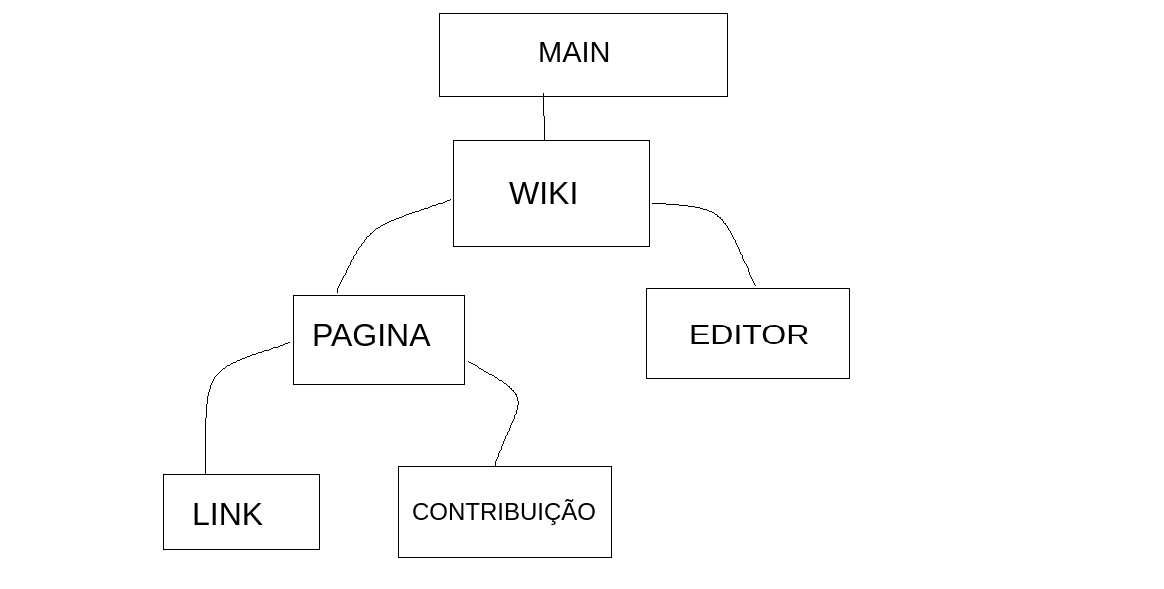
\includegraphics[width=0.8\textwidth]{estrutura.png}
    \caption{Hierarquia geral do projeto.}
    \label{img:hierarquia}
\end{figure}

\chapter{Conclusão}
De modo geral, o trabalho apresentou desafios relativamente simples, fazendo
com que outras questões tomassem maior tempo. Etapas como organização de código
e planejamento de estruturas é algo que se feito errado pode trazer
complicações futuras para o programa. A adoção de ferramentas como Valgrind se
faz quase que necessário para poder cuidar de todos as nuances do projeto.

\phantompart

\bibliography{main}

\end{document}
